\begin{figure}[H]
	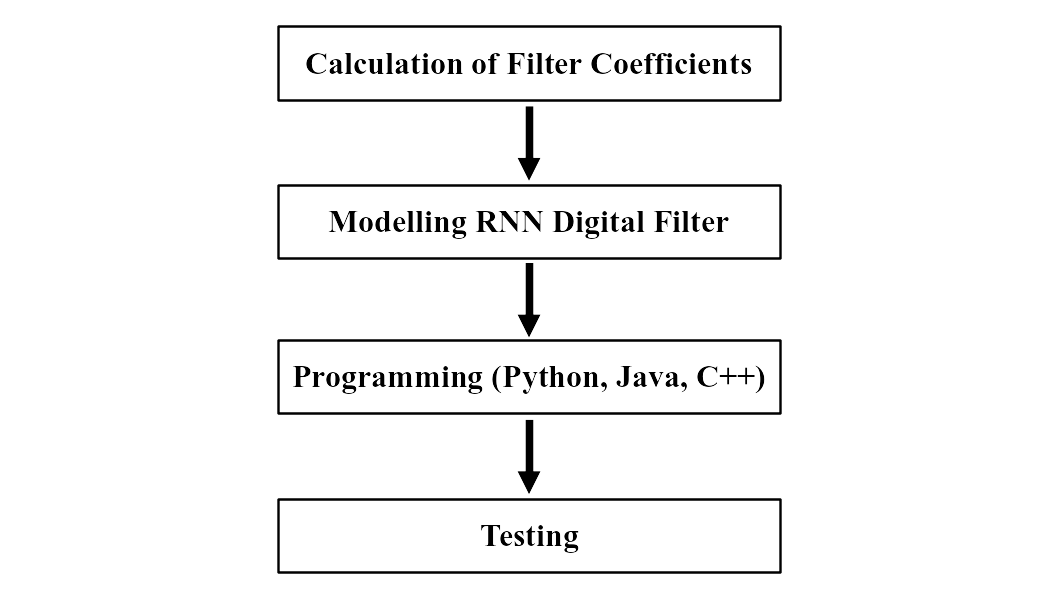
\includegraphics[width=\columnwidth, keepaspectratio]{methodology}
	\caption{Steps Followed in Implementation}
	\label{Fig:fig1}
\end{figure}

\subsection*{1. Calculation of Filter Coefficients:}
\begin{itemize}
	\item Define specifications and select a design method.
	\item Formulate math expressions, compute coefficients, and verify accuracy.
	\item Document coefficients and adjustments.
\end{itemize}

\subsection*{2. Modelling of RNN Digital Filter:}
\begin{itemize}
	\item Choose RNN architecture (e.g., LSTM).
	\item Define input/output layers and integrate filter coefficients.
	\item Prepare training data for RNN.
\end{itemize}

\subsection*{3. Programming (Python, Java, C++):}
\begin{itemize}
	\item Choose a language (e.g., Python with TensorFlow).
	\item Implement filter coefficients and RNN model.
\end{itemize}

\subsection*{4. Testing:}
\begin{itemize}
	\item Generate diverse test datasets.
	\item Evaluate RNN filter performance using metrics.
	\item Refine model iteratively if needed.
	\item Document test results for future reference.
\end{itemize}